\documentclass[conference,10pt]{IEEEtran}

\usepackage[utf8]{inputenc}
\usepackage[T1]{fontenc}
\usepackage{amsmath,amssymb}
\usepackage{graphicx}
\usepackage{booktabs}
\usepackage{multirow}
\usepackage{xcolor}
\usepackage{hyperref}
\usepackage{cleveref}
\usepackage{tikz}
\usetikzlibrary{arrows.meta,positioning,shapes.geometric,fit,calc}
\usepackage{enumitem}
\usepackage{balance}
\usepackage{url}
\usepackage{array}
\usepackage{tabularx}
\usepackage{makecell}
\usepackage{pifont}

\hypersetup{
  colorlinks=true,
  linkcolor=blue!70!black,
  citecolor=blue!70!black,
  urlcolor=blue!70!black
}
\usepackage{xurl}

\newcommand{\ie}{\textit{i.e.}}
\newcommand{\eg}{\textit{e.g.}}
\newcommand{\cf}{\textit{cf.}}
\newcommand{\etal}{\textit{et~al.}}
\newcommand{\vcf}{\textsc{vcf}}

\begin{document}

\title{Visual Cryptographic Fingerprints\\for AI Supply-Chain Identity}

\author{
  \IEEEauthorblockN{Shubham Kumar}
  \IEEEauthorblockA{Independent Researcher\\
  shubhambtps@live.in}
}

\maketitle

% ============================================================
\begin{abstract}
AI systems increasingly depend on third-party models, datasets, and training pipelines distributed through open ecosystems, creating supply-chain risks that have materialized in real attacks---from malicious pickle payloads on Hugging Face to transferable backdoors in pre-trained models.
In response, the community has built machine-verifiable provenance infrastructure: cryptographic model signing (OpenSSF~OMS, Sigstore), attestation frameworks (in-toto, SLSA), and AI Bills of Materials (AIBOMs).
However, a critical usability gap remains: when human operators must verify artifact identity---at deployment gates, during incident response, or while browsing model registries---they face long hexadecimal hashes that decades of usability research show humans compare poorly, and that attackers can exploit through partial matching and perceptual similarity.

This paper systematically maps \emph{visual cryptographic fingerprints} to AI supply-chain identity.
We systematize ten existing visual hash schemes against security, usability, and accessibility criteria; define a threat model for AI artifact identity covering both exact and perceptual collisions; and propose an integration architecture that composes visual fingerprints with model signing, AIBOMs, and transparency logs.
We also implement a reference prototype of three encoding families, report collision and near-collision measurements on 100K samples, and lay out open challenges---chief among them the need for human-subject validation before any production deployment.
Visual fingerprints are not a replacement for cryptographic verification---they reduce human error at the decision points where tooling is imperfect or bypassed entirely.
\end{abstract}

\begin{IEEEkeywords}
  hash visualization, visual fingerprints, AI supply chain, model provenance, model signing, perceptual collision resistance
\end{IEEEkeywords}

% ============================================================
\section{Introduction}
\label{sec:intro}

The AI supply chain has become a primary attack vector.
In 2024--2025, security researchers documented weaponized PyTorch model files on Hugging Face that executed embedded shell commands to deploy remote access trojans upon loading via \texttt{torch.load()}~\cite{cso2025pickle,rapid72025pickle}.
A critical vulnerability in the vllm inference library (CVE-2025-24357) allowed remote code execution through malicious pickle deserialization of model weights downloaded from public registries~\cite{vllm2025cve}.
TransTroj demonstrated that pre-trained model backdoors can be designed to survive fine-tuning, enabling supply-chain poisoning that propagates through the entire downstream ecosystem~\cite{transtroj2025www}.

The community has responded with machine-verifiable provenance infrastructure---and the progress is real.
Sigstore's model-transparency project reached v1.0 in 2025, providing cryptographic signing for ML models with identity binding and transparency logging~\cite{sigstore2025model}.
The OpenSSF Model Signing (OMS) specification aims to standardize signing across ML frameworks~\cite{openssf2025oms}.
SLSA provides incremental supply-chain security levels with provenance attestation formats~\cite{slsa2023spec}.
AI Bills of Materials (AIBOMs) based on CycloneDX document model lineage with cryptographic validation~\cite{aibom2026frontiers,owasp2025aibom}.
The EU AI Act mandates provenance traceability and human oversight for high-risk AI systems, with full enforcement beginning in August~2026~\cite{euaiact2024}.

Yet these systems share a conspicuous \emph{usability gap}.
When a human operator must verify an artifact's identity---approving a model deployment, triaging an incident, or reviewing a model card---they face identifiers like \texttt{SHA256:b3f8d9ac\-fa99\-13...}.
A 25-year research record demonstrates that humans compare such strings poorly.
Dechand~\etal~conducted a 1,047-participant study and found hexadecimal is the representation most vulnerable to partial-preimage attacks~\cite{dechand2016empirical}.
Tan~\etal~showed attack success rates ranging from 6\% to 72\% across fingerprint representations under realistic conditions with habituation and distraction~\cite{tan2017unicorns}.

\emph{Visual cryptographic fingerprints}---deterministic images derived from cryptographic digests---are one way to close this gap.
The idea traces to Perrig and Song's hash visualization formalism~\cite{perrig1999hash} and was deployed in OpenSSH's randomart feature~\cite{openssh2008release}.
But applying this concept to AI supply chains is harder than it looks.
Model registries contain tens of thousands of artifacts across diverse types (weights, datasets, adapters, pipelines), the visual layer must integrate with existing provenance stacks, and---most importantly---the encoding must resist \emph{perceptual} collision mining by well-funded adversaries.

\subsection{Contributions}

Our contributions are:

\begin{enumerate}[leftmargin=*,nosep]
  \item A \textbf{taxonomy of ten visual hash schemes} evaluated against security, usability, and accessibility criteria drawn from empirical literature (\Cref{sec:systematization}).
  \item A \textbf{threat model} covering exact and perceptual collisions under realistic attacker budgets (\Cref{sec:threat}).
  \item An \textbf{integration architecture} that binds visual fingerprints to model signing (OMS, Sigstore), AIBOMs (CycloneDX), and transparency logs---not just artifact hashes (\Cref{sec:architecture}).
  \item A \textbf{reference prototype} of three encoding families with empirical collision and near-collision measurements on 100K samples (\Cref{sec:analysis}).
  \item A \textbf{research agenda} centered on the human-subject validation that must precede any deployment (\Cref{sec:discussion}).
\end{enumerate}

To be clear: visual fingerprints do not replace machine verification. They fill a narrow but real gap---human decision points where tooling is imperfect, bypassed, or absent.

% ============================================================
\section{Background}
\label{sec:background}

\subsection{Hash Visualization}

Perrig and Song~\cite{perrig1999hash} formalized Hash Visualization Algorithms (HVAs) in 1999, defining security properties that explicitly incorporate human perception.
Beyond standard collision resistance, they introduced \emph{near collision resistance}---the requirement that it be computationally difficult to find two inputs whose visual outputs are perceptually indistinguishable to a human observer---and \emph{near one-wayness}---the difficulty of finding an input whose visual output matches a target image.
Their ``Random Art'' prototype generates abstract images from mathematical expression trees seeded by a hash digest.
This framing remains a useful security model for visual identity: the cryptographic hash provides binding to artifact identity; the visual layer is a perceptual compression that must be analyzed as such.

\subsection{OpenSSH Randomart}

OpenSSH added an experimental ASCII fingerprint visualization feature (VisualHostKey) in version~5.1 (2008), explicitly citing Perrig and Song~\cite{openssh2008release}.
The algorithm---later analyzed as the ``drunken bishop'' by Loss~\etal~\cite{loss2009drunken}---performs a bounded random walk on a 17$\times$9 grid driven by bit-pairs from the fingerprint digest.
Visit counts are mapped to an ASCII character ramp.
Loss~\etal\ raised the question of whether the scheme is ``secure enough,'' noting that Markov analysis and brute-force collision exploration reveal structural properties that could be exploited.
Despite these open questions, the feature remains deployed in production OpenSSH with no formal security guarantees for its visual output.

\subsection{Key Fingerprint Usability Studies}

Four landmark studies inform the design space for visual fingerprints:

\begin{itemize}[leftmargin=*,nosep]
  \item \textbf{Hsiao~\etal~(ACSAC~2009)}~\cite{hsiao2009study} compared Base32, Random Art, and Flag-based schemes, reporting accuracy and time across ``easy'' and ``hard'' comparison pairs. They noted that visual schemes require sufficient display resolution and highlighted entropy limits (20--30~bits typically displayed).
  \item \textbf{Dechand~\etal~(USENIX Security~2016)}~\cite{dechand2016empirical} conducted a 1,047-participant study comparing textual fingerprint encodings. Their central finding: hexadecimal is more vulnerable to partial-preimage attacks than alternatives. Sentence-based encodings achieved the best attack detection rate and usability perception; numeric encodings are a practical fallback.
  \item \textbf{Tan~\etal~(CHI~2017)}~\cite{tan2017unicorns} studied eight fingerprint representations with 661~participants under habituation and distraction, modeling attackers who generate many candidates and select the most similar. Attack success ranged from 6\% (best case) to 72\% (worst case) across representations.
  \item \textbf{Azimpourkivi~\etal~(USENIX Security~2020)}~\cite{azimpourkivi2020human} formalized \emph{strong} versus \emph{weak} Visual Key Fingerprint Generators (VKFGs). Their CEAL system uses error-correcting codes (ECC) to enforce minimum Hamming distance in the input space, combined with a neural generator, and introduces the Human Perception Distinguishability ratio (HPD\textsubscript{ratio}) to formally target perceptual collision resistance.
\end{itemize}

\subsection{AI Supply Chain Security Primitives}
\label{sec:bg:supplychain}

Modern AI supply-chain security builds on several complementary frameworks:

\noindent\textbf{in-toto}~\cite{torres2019intoto} provides end-to-end supply-chain integrity by having project owners declare a signed ``layout'' of build steps and generating signed ``link metadata'' at each step, binding inputs and outputs to authorized actors.

\noindent\textbf{Sigstore}~\cite{sigstore2024docs} provides keyless signing with ephemeral keys, binding signatures to identities via OIDC, and recording signing events in an append-only transparency log (Rekor).

\noindent\textbf{SLSA}~\cite{slsa2023spec} defines incremental supply-chain security levels with standardized provenance and attestation formats.

\noindent\textbf{OpenSSF Model Signing}~\cite{openssf2025oms} (OMS, 2025) extends these practices to ML models, providing a standards-based signing specification compatible with Sigstore and major ML frameworks.

\noindent\textbf{AIBOMs}~\cite{aibom2026frontiers,owasp2025aibom} (AI Bills of Materials) extend CycloneDX to document model lineage, training data provenance, and dependencies with cryptographic validation.

What is missing from this stack is a \emph{human-facing identity layer}---something that lets an operator recognize an artifact at a glance while the underlying provenance and signatures remain machine-verifiable.

% ============================================================
\section{Systematization of Visual Hash Schemes}
\label{sec:systematization}

We survey ten visual hash schemes spanning 25~years of development, evaluating each against criteria derived from the empirical literature (\Cref{tab:taxonomy}).
Schemes were selected by searching the academic literature (Google Scholar, ACM DL, IEEE Xplore) for ``hash visualization,'' ``visual fingerprint,'' and ``visual identity,'' supplemented by deployed systems found in open-source repositories (GitHub, npm, crates.io).
We included every scheme we could find with either a published description or an open-source implementation; schemes that are purely proprietary or undocumented were excluded.
Ratings were assigned by the author based on published analyses where available and on documented properties of the implementation otherwise; a~``?'' indicates no evidence was found.
Our evaluation dimensions are:

\begin{itemize}[leftmargin=*,nosep]
  \item \textbf{Determinism}: Identical input always produces identical output.
  \item \textbf{Visual salience}: Magnitude of perceptible change when the input changes.
  \item \textbf{Near-preimage resistance}: Difficulty of finding an input whose visual output appears similar to a target under realistic attacker budgets.
  \item \textbf{Formal analysis}: Whether security properties have been formally analyzed or empirically measured.
  \item \textbf{Device robustness}: Stability under scaling, screenshotting, and grayscale printing.
  \item \textbf{Accessibility}: Suitability for users with color vision deficiency (${\sim}$8\% of males), availability of non-color fallbacks.
  \item \textbf{Deployment status}: Research prototype versus production deployment.
\end{itemize}

\smallskip\noindent\textbf{Rating rubric.}
\emph{Near-preimage resistance:} High~=~formal analysis or human-distinguishability design; Low~=~partial inputs or documented mineability; ?~=~no evidence.
\emph{Device robustness:} High~=~monochrome/ASCII, resilient to scaling; Low~=~color-dependent.
\emph{Accessibility:} High~=~usable without color; Low~=~color-primary with no fallback.

\begin{table*}[t]
\centering
\caption{Taxonomy of Visual Hash Schemes. Criteria derived from Perrig \& Song~\cite{perrig1999hash}, Hsiao~\etal~\cite{hsiao2009study}, Dechand~\etal~\cite{dechand2016empirical}, Tan~\etal~\cite{tan2017unicorns}, and Azimpourkivi~\etal~\cite{azimpourkivi2020human}. Ratings assigned by the author per the rubric above. Legend: \ding{51}\,=\,yes/strong, $\sim$\,=\,partial/medium, \ding{55}\,=\,no/weak, ?\,=\,unknown/untested.}
\label{tab:taxonomy}
\small
\renewcommand{\arraystretch}{1.15}
\begin{tabular}{@{}l c c c c c c c c@{}}
\toprule
\textbf{Scheme} & \textbf{Year} & \textbf{Encoding Style} & \textbf{Determ.} & \makecell{\textbf{Near-Preimage}\\\textbf{Resistance}} & \makecell{\textbf{Formal}\\\textbf{Analysis}} & \makecell{\textbf{Device}\\\textbf{Robust.}} & \textbf{Access.} & \textbf{Deployed} \\
\midrule
Random Art~\cite{perrig1999hash} & 1999 & Expression trees & Yes & ? & Partial & $\sim$ & $\sim$ & Research \\
SSH Randomart~\cite{openssh2008release,loss2009drunken} & 2008 & Random walk grid & Yes & $\sim$ & Partial & High & High & Production \\
Identicons~\cite{github2013identicons} & 2007 & 5$\times$5 pixel sprite & Yes & Low & No & $\sim$ & $\sim$ & Production \\
Chroma-Hash~\cite{chromahash2009} & 2009 & Color-bar strip & Yes & Low & No & Low & Low & Prototype \\
VizHash GD~\cite{vizhash2012} & 2012 & Layered shapes & Yes & ? & No & $\sim$ & $\sim$ & Prototype \\
Eth.\ Blockies & 2015 & Low-res pixel grid & Yes & Low & No & $\sim$ & $\sim$ & Production \\
CEAL~\cite{azimpourkivi2020human} & 2020 & ECC + neural gen. & Yes & \textbf{High} & \textbf{Yes} & $\sim$ & ? & Research \\
Mosaic Hash~\cite{fietkau2020mosaic} & 2020 & Circle segments & Yes & ? & Partial & $\sim$ & $\sim$ & Prototype \\
LifeHash~\cite{lifehash2021} & 2021 & Cellular automata & Yes & ? & No & $\sim$ & $\sim$ & Production \\
MetaMask Jazzicon & 2016 & Color collage & Yes & Low & No & Low & Low & Production \\
\bottomrule
\end{tabular}
\end{table*}

\subsection{Key Findings from Systematization}

\noindent\textbf{Most schemes lack formal security analysis.}
Of the ten schemes surveyed, only CEAL~\cite{azimpourkivi2020human} provides formal human-distinguishability guarantees through its ECC-enforced minimum distance and HPD\textsubscript{ratio} metric.
The OpenSSH randomart analysis by Loss~\etal~\cite{loss2009drunken} provides partial formal treatment but explicitly questions whether the scheme is ``secure enough.''
All other schemes have no published security analysis of their perceptual collision properties.

\noindent\textbf{Identicons use partial input, creating a mineable attack surface.}
GitHub identicons are derived from a hash of the user ID, and Ethereum blockies/Jazzicon operate on addresses with known prefix constraints.
MetaMask contributors explicitly documented the risk of ``mineable'' identicons when only a partial address is used as input~\cite{metamask2016identicon}.
This is directly relevant to AI supply chains, where model names or short identifiers might be used instead of full cryptographic digests.

\noindent\textbf{Color dependency limits accessibility and robustness.}
Schemes relying primarily on color differentiation (Chroma-Hash, Jazzicon, some LifeHash configurations) are vulnerable to both accessibility failures (color vision deficiency) and device variability (color management differences across displays and printers).
Hsiao~\etal~\cite{hsiao2009study} specifically warned that schemes requiring color and high-resolution displays limit deployability.

\noindent\textbf{No scheme was designed for AI supply-chain contexts.}
All surveyed schemes target SSH keys, password fields, cryptocurrency addresses, or general-purpose visual hashing.
AI artifact identity is materially different for several reasons: (1)~the object of identity is not a single key but a heterogeneous bundle of weights, adapters, tokenizers, datasets, and pipeline configurations; (2)~identity must incorporate provenance state (who signed it, what attestations exist), not just a file hash; (3)~registries contain tens of thousands of entries, so visual fingerprints will be encountered at browsing scale, not one at a time; and (4)~operators typically encounter artifacts through web UIs and deployment gates rather than raw CLI verification.
These constraints make direct transplantation of existing schemes insufficient.

% ============================================================
\section{Threat Model}
\label{sec:threat}

We consider an adversary targeting the identity-verification step in an AI supply-chain workflow.
The defender maintains a trusted reference identity (a pinned expected digest from a signed release) and receives a candidate identity from a downloaded or registry-served artifact.
Verification involves both machine checks (signature and provenance policy enforcement) and a human check at a UI decision point.

\subsection{Threat Scenarios}

We ground our threat model in documented incidents:

\begin{enumerate}[leftmargin=*,nosep]
  \item \textbf{Model substitution.} The attacker replaces a model file in a registry or in transit with a malicious version. This is the attack pattern documented in Hugging Face pickle exploits~\cite{cso2025pickle,rapid72025pickle} and the vllm vulnerability~\cite{vllm2025cve}.
  \item \textbf{Checkpoint poisoning.} The attacker publishes a pre-trained model with an embedded backdoor designed to survive fine-tuning, as demonstrated by TransTroj~\cite{transtroj2025www}.
  \item \textbf{Dataset tampering.} Training or evaluation data is modified to influence model behavior, a well-documented attack class~\cite{backdoor2025survey}.
  \item \textbf{Rollback/version confusion.} An older but validly signed artifact is served instead of the expected current version.
  \item \textbf{Attestation mismatch.} A validly signed artifact is paired with provenance metadata from a different artifact or pipeline.
\end{enumerate}

\subsection{Attacker Capabilities}

\begin{itemize}[leftmargin=*,nosep]
  \item \textbf{A1 (Substitution):} Replace artifacts in transit or in a compromised registry. Machine verification (signature checks) blocks this unless the attacker also controls signing keys.
  \item \textbf{A2 (Near-preimage mining):} Generate $M$ candidate artifacts and select the one whose visual fingerprint maximizes similarity to a target. Following Tan~\etal~\cite{tan2017unicorns}, we model budgets $M \in \{2^{20}, 2^{24}, 2^{28}\}$ for commodity to well-funded adversaries.
  \item \textbf{A3 (Habituation exploitation):} Exploit human inattention during routine approval workflows where the vast majority of artifacts are legitimate, leading to ``rubber-stamping.'' Tan~\etal\ measured this effect explicitly.
  \item \textbf{A4 (UI spoofing):} Present a forged or misleading visual fingerprint in a compromised UI, bypassing the visual comparison entirely.
\end{itemize}

\subsection{Defender Model}

The defender deploys:
\begin{itemize}[leftmargin=*,nosep]
  \item \textbf{Machine verification:} Signature validation, provenance policy checks, transparency log verification---enforced by tooling (Sigstore cosign, in-toto verification, SLSA policy engines).
  \item \textbf{Human verification:} Visual comparison at decision points---deployment approval gates, model card review, incident triage, cross-team communication.
  \item \textbf{Visual fingerprint:} A deterministic image derived from a \emph{signed bundle digest} (defined in \Cref{sec:architecture}), displayed alongside machine verification results.
\end{itemize}

\subsection{Goals and Non-Goals}

The visual fingerprint lives in the gap between ``machine verification passed'' and ``human must still approve.''
That gap is real: organizations require human sign-off for model deployments, and machine verification can be misconfigured, incomplete, or quietly overridden by someone running \texttt{-{}-skip-verify}.

\smallskip\noindent\textbf{Goals:} (G1)~Reduce human comparison error at authenticated decision points where a trusted reference VCF exists. (G2)~Aid recognition and change detection for artifacts a user has seen before.

\smallskip\noindent\textbf{Non-goals:} VCFs do not defend against compromised UIs (A4 requires a trusted rendering path, which we assume but do not construct). They do not replace signature or provenance enforcement. They are not a search mechanism for large registries.

% ============================================================
\section{Integration Architecture}
\label{sec:architecture}

We propose an architecture that composes visual cryptographic fingerprints (VCFs) with existing AI supply-chain infrastructure, ensuring that the visual identity is bound to the full provenance chain rather than the artifact hash alone.

\subsection{Bundle Digest Derivation}

A VCF is defined as a deterministic function of a \emph{bundle digest}:

\begin{equation}
\label{eq:bundle}
\texttt{Bundle} = (h_a,\; \sigma,\; \textit{id}_s,\; \alpha,\; \pi)
\end{equation}

\noindent where $h_a$ is the artifact digest (\eg, SHA-256 of model weights), $\sigma$ is the cryptographic signature, $\textit{id}_s$ is the signer identity (OIDC subject from Sigstore), $\alpha$ is the attestation/provenance metadata, and $\pi$ is the transparency log inclusion proof.
These are logical fields, not raw tool output; a production specification would need to fix exact field extraction and normalization rules so that two independent verifiers derive the same bundle from the same signing event.

The bundle digest is computed as:
\begin{equation}
\label{eq:bundledigest}
\texttt{BD} = \text{SHA-256}(\text{JCS}(\texttt{Bundle}))
\end{equation}

\noindent where JCS denotes JSON Canonicalization Scheme (RFC~8785) to ensure deterministic serialization.
The visual fingerprint is then:
\begin{equation}
\label{eq:vcf}
\texttt{VCF} = \text{Render}(\text{Encode}(\texttt{BD}),\; v_{\text{spec}})
\end{equation}

\noindent where $v_{\text{spec}}$ is a version identifier for the rendering specification to ensure cross-platform determinism.

This design means that any change to the artifact, signature, signer identity, provenance, or log proof changes the visual output.
An attacker who substitutes a model must either (a)~forge a valid bundle or (b)~find a substitute whose bundle digest produces a perceptually similar visual output.

\smallskip\noindent\textbf{Stability caveat.}
Including the transparency-log proof~$\pi$ in the bundle creates a tension: if~$\pi$ can change over time (e.g., due to log compaction or proof format updates), the VCF changes even though the artifact has not.
A production design must either pin~$\pi$ at signing time or exclude it from the VCF input and verify it separately.
We flag this as an open engineering decision.

\subsection{Integration Points}

\Cref{fig:architecture} illustrates the end-to-end flow.
VCFs integrate at five points in existing AI workflows:

\begin{enumerate}[leftmargin=*,nosep]
  \item \textbf{Model registries:} Thumbnail VCF alongside each model entry, enabling visual browsing and anomaly detection.
  \item \textbf{Model cards / AIBOMs:} Embedded VCF in documentation artifacts, providing a visual anchor for provenance records~\cite{aibom2026frontiers}.
  \item \textbf{Deployment gates:} Side-by-side comparison of expected VCF (from release manifest) and candidate VCF (from downloaded artifact) during approval workflows.
  \item \textbf{CLI tools:} ASCII randomart output in terminal signing/verification workflows, analogous to SSH VisualHostKey.
  \item \textbf{Incident response:} Quick visual identification of which model version is deployed, without requiring hash string comparison.
\end{enumerate}

\begin{figure}[t]
\centering
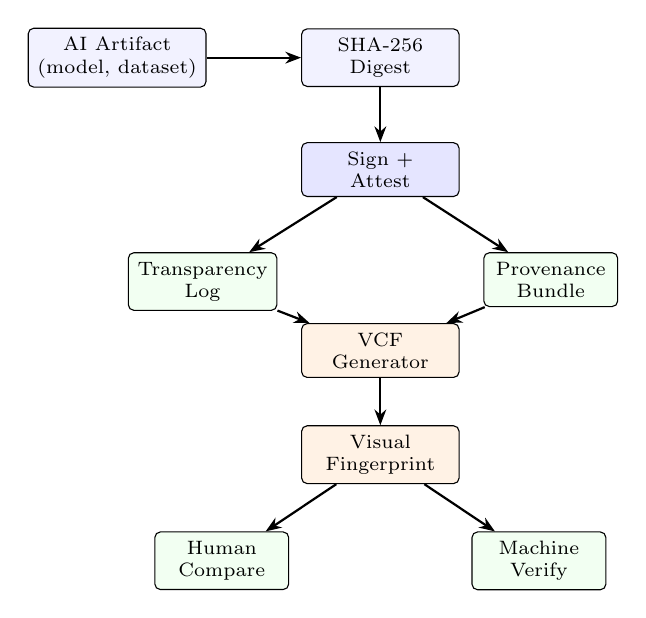
\begin{tikzpicture}[
  node distance=0.6cm and 0.7cm,
  box/.style={draw, rounded corners=2pt, minimum width=2cm, minimum height=0.55cm, font=\scriptsize, align=center, fill=blue!5},
  smallbox/.style={draw, rounded corners=2pt, minimum width=1.7cm, minimum height=0.5cm, font=\scriptsize, align=center, fill=green!5},
  genbox/.style={draw, rounded corners=2pt, minimum width=2cm, minimum height=0.55cm, font=\scriptsize, align=center, fill=orange!10},
  arr/.style={-{Stealth[length=2mm]}, thick},
]
  % Row 1: Artifact and Hash
  \node[box] (artifact) {AI Artifact\\(model, dataset)};
  \node[box, right=1.2cm of artifact] (hash) {SHA-256\\Digest};

  % Row 2: Sign + Attest (centered under hash)
  \node[box, below=0.7cm of hash, fill=blue!10] (sign) {Sign +\\Attest};

  % Row 3: Transparency Log and Provenance Bundle
  \node[smallbox, below left=0.7cm and 0.3cm of sign] (tlog) {Transparency\\Log};
  \node[smallbox, below right=0.7cm and 0.3cm of sign] (prov) {Provenance\\Bundle};

  % Row 4: VCF Generator (centered)
  \node[genbox, below=1.6cm of sign] (vcfgen) {VCF\\Generator};

  % Row 5: Visual Fingerprint
  \node[genbox, below=0.6cm of vcfgen] (vcf) {Visual\\Fingerprint};

  % Row 6: Human and Machine (flanking VCF output)
  \node[smallbox, below left=0.6cm and 0.15cm of vcf] (human) {Human\\Compare};
  \node[smallbox, below right=0.6cm and 0.15cm of vcf] (machine) {Machine\\Verify};

  % Arrows: top-down flow
  \draw[arr] (artifact) -- (hash);
  \draw[arr] (hash) -- (sign);
  \draw[arr] (sign) -- (tlog);
  \draw[arr] (sign) -- (prov);
  \draw[arr] (tlog) -- (vcfgen);
  \draw[arr] (prov) -- (vcfgen);
  \draw[arr] (vcfgen) -- (vcf);
  \draw[arr] (vcf) -- (human);
  \draw[arr] (vcf) -- (machine);
\end{tikzpicture}
\caption{Integration architecture: a Visual Cryptographic Fingerprint (VCF) is derived from the full signed provenance bundle, not the artifact hash alone. Machine verification and human visual comparison operate in parallel.}
\label{fig:architecture}
\end{figure}

\subsection{Compatibility with Existing Standards}

\noindent\textbf{OpenSSF Model Signing (OMS):} The bundle digest is derived from the signed model artifact plus OMS metadata, making the VCF a deterministic function of the signing event.

\noindent\textbf{Sigstore model-transparency:} The VCF generator consumes cosign verification output (signature, certificate, Rekor entry) to construct the bundle.

\noindent\textbf{CycloneDX AIBOMs:} A VCF reference (image or ASCII) can be embedded in the \texttt{component.properties} section of an AIBOM document.

\noindent\textbf{in-toto:} For multi-step pipelines, VCFs can be derived from individual step link metadata or from the aggregate layout verification result, providing visual identity at multiple granularity levels.

\subsection{Candidate Encoding Families}

We narrow the design space to three encoding families, implemented as a reference prototype (\Cref{sec:analysis}).

\subsubsection{Encoding~A: Random-Walk Grid}
Interprets bit-pairs of the bundle digest as diagonal directions on a bounded grid, incrementing visit counters.
Visit counts are mapped to an ASCII character ramp.
Based on the drunken bishop algorithm~\cite{loss2009drunken}, adapted to SHA-256 (256~bits $\rightarrow$ 128~moves).

\smallskip\noindent\textit{Strengths:} Terminal-friendly, extremely low computational cost ($O(|D|)$), well-understood by SSH users.
\textit{Weaknesses:} Limited perceptual entropy; users may focus on gross shape only; Loss~\etal\ raised security concerns.
\textit{Best pairing:} Sentence-based textual encoding as recommended by Dechand~\etal~\cite{dechand2016empirical}.

\subsubsection{Encoding~B: Cellular Automata (LifeHash-like)}
Seeds a cellular automaton with digest bits, evolves for $T$~steps, and renders the accumulated state with optional symmetry enforcement.
LifeHash~\cite{lifehash2021} is an existence proof that this approach produces aesthetically appealing, recognizable patterns.

\smallskip\noindent\textit{Strengths:} High visual entropy; symmetry aids recognition; can be designed for grayscale robustness.
\textit{Weaknesses:} Parameter sensitivity (grid size, step count, CA rule); some configurations collapse to stable attractors, reducing effective output diversity.
\textit{Best pairing:} Model cards and registry UIs where graphical display is standard.

\subsubsection{Encoding~C: Voronoi Tessellation}
Derives $K$ site points from the digest, partitions the image plane by nearest-site distance, and colors each cell from a stable palette.

\smallskip\noindent\textit{Strengths:} High salience for moderate $K$; produces distinctive region shapes.
\textit{Weaknesses:} Color-dependent (accessibility concern); palette compression can mask differences.
Hsiao~\etal~\cite{hsiao2009study} warned that excessive visual complexity can reduce comparison accuracy.
\textit{Best pairing:} Dashboard displays where graphical richness aids recognition; must include colorblind-safe palette.

\subsection{Example: Legitimate vs.\ Tampered Model}

\Cref{fig:ascii} shows random-walk VCFs generated by our prototype from SHA-256 digests of two model identifiers differing by a single suffix.
In a production system, the input would be a full bundle digest (\Cref{sec:architecture}), not a bare name; we use identifiers here to illustrate encoding behavior.
The resulting patterns are visibly different.

\begin{figure}[t]
\centering
\small
\begin{verbatim}
  llama3-70b-v1       llama3-70b-v1
    (original)          (tampered)
+--[SHA256]------+  +--[SHA256]------+
|+=+=. .         |  |.o***.o.        |
|B*=oo*..        |  | o+=.=o. .      |
|.**=*oo o . .   |  |.+..+o o+ .     |
|.+.o+o o . . .  |  |..o o+.o.+      |
|. . . . S   .   |  |  o.o o S .     |
|   o.  = . .    |  | + . + . . +    |
|  ....+   .     |  |  = . = o = .   |
|...  ..o .      |  | . . + o o .    |
|=.     .o       |  |  ..o...o       |
+----------------+  +----------------+
\end{verbatim}
\caption{Random-walk VCF output for two different SHA-256 inputs, illustrating deterministic rendering. This is not evidence of resistance to attacker-mined similarity; it shows the encoding's visual style and the avalanche property of the underlying hash.}
\label{fig:ascii}
\end{figure}

% ============================================================
\section{Prototype Implementation and Empirical Evaluation}
\label{sec:analysis}

We implement a reference prototype of all three encoding families and conduct automated collision and near-collision testing.
Our prototype is a Python library ({\raise.17ex\hbox{$\scriptstyle\sim$}}350 LOC) using NumPy, SciPy, Pillow, scikit-image, and ImageHash.
All experiments use 64$\times$64 grayscale renderings and SHA-256 digests from cryptographically random 256-bit inputs.
Parameter choices (17$\times$9 grid, 32$\times$32 CA board, 8 evolution steps, 16 Voronoi sites, 64$\times$64 render resolution) are exploratory settings chosen to balance visual recognizability and computational cost; they are not optimized designs and different values may yield different trade-offs.

\subsection{Encoding Implementations}

\subsubsection{Random-Walk Grid}
We implement the drunken bishop algorithm~\cite{loss2009drunken} on a 17$\times$9 grid.
Each SHA-256 byte yields four 2-bit direction pairs (128 moves total).
Visit counts are rendered both as ASCII (17-character ramp) and as a grayscale image via nearest-neighbor upscaling.

\subsubsection{Cellular Automata}
A 32$\times$32 Game-of-Life grid is seeded from the 256 digest bits (with horizontal symmetry enforced for recognizability, following LifeHash~\cite{lifehash2021}).
The board evolves for 8 steps; the accumulated ``heat map'' of cell activations is rendered as a grayscale image.

\subsubsection{Voronoi Tessellation}
Sixteen site points are derived from the digest (one byte each for $x$ and $y$ coordinates), and the image plane is partitioned by nearest-site distance.
Cell intensities are assigned from a deterministic lookup table seeded by remaining digest bytes.

\subsection{Exact Collision Testing}

We generated 100,000 random SHA-256 digests, rendered each through all three encodings, and checked for exact output collisions by hashing the pixel bytes (SHA-256 of the rendered image).

\begin{table}[t]
\centering
\caption{Exact collision testing results ($N{=}100{,}000$ random SHA-256 digests, 64$\times$64 grayscale renderings). Zero exact collisions were found for any encoding.}
\label{tab:exact}
\small
\renewcommand{\arraystretch}{1.15}
\begin{tabular}{@{}l r r r@{}}
\toprule
\textbf{Encoding} & \textbf{Unique Outputs} & \textbf{Collisions} & \textbf{Render Rate} \\
\midrule
Random-walk & 100,000 & 0 & 14,769/s \\
Cellular auto. & 100,000 & 0 & 3,446/s \\
Voronoi & 100,000 & 0 & 3,337/s \\
\bottomrule
\end{tabular}
\end{table}

\Cref{tab:exact} shows zero exact collisions across all 100,000 samples for every encoding.
While this is expected (the output spaces are far larger than $10^5$), it confirms the implementations are not degenerate and produce fully distinct outputs for distinct inputs.

\subsection{Near-Collision Analysis}

Exact collisions are not the primary risk---perceptual near-collisions are~\cite{tan2017unicorns}.
We measure two automated similarity metrics across 10,000 random pairs per encoding:
\textbf{SSIM} (Structural Similarity Index, range $[-1, 1]$, higher $=$ more similar) and
\textbf{pHash distance} (perceptual hash Hamming distance, lower $=$ more similar; a 64-bit hash yields max distance 64).

\begin{table}[t]
\centering
\caption{Near-collision analysis: similarity between random pairs (10K pairs) and targeted mining (20 targets $\times$ 2K candidates). SSIM $>$ 0.9 and pHash distance $<$ 5 are typical ``perceptually similar'' thresholds.}
\label{tab:collision}
\footnotesize
\renewcommand{\arraystretch}{1.15}
\begin{tabular}{@{}l c c c c@{}}
\toprule
& \multicolumn{2}{c}{\textbf{Random Pairs}} & \multicolumn{2}{c}{\textbf{Mining ($M{=}2{,}000$)}} \\
\cmidrule(lr){2-3} \cmidrule(lr){4-5}
\textbf{Encoding} & \makecell{SSIM\\mean / max} & \makecell{pHash\\mean / min} & \makecell{Best\\SSIM} & \makecell{Best\\pHash} \\
\midrule
Random-walk & 0.18 / 0.68 & 31.4 / 12 & 0.72 & 12 \\
Cellular & 0.02 / 0.16 & 15.3 / 5 & 0.19 & 4 \\
Voronoi & 0.22 / 0.48 & 31.5 / 18 & 0.45 & 16 \\
\bottomrule
\end{tabular}
\end{table}

The results in \Cref{tab:collision} split cleanly along encoding complexity.
The random-walk grid is the weakest: even 2,000 mining attempts yield a pair at SSIM 0.72, well into ``looks similar'' territory.
This is not surprising---Loss~\etal~\cite{loss2009drunken} already questioned whether a 17$\times$9 grid constrains output diversity too much, and our numbers confirm that worry.
On its own, random-walk appears inadequate as a stand-alone visual cue; pairing it with a sentence-based textual encoding~\cite{dechand2016empirical} is the minimum.

Cellular automata are a different story.
Random-pair SSIM averages 0.02---effectively uncorrelated---and the best match an attacker finds in 2,000 tries is SSIM 0.19, well below the levels we observe for the other two encodings under the same metrics.
Whether 0.19 would confuse a human is an open question that requires the study proposed in \Cref{sec:discussion}, but the gap between encodings is clear.

Voronoi sits in between (mining best SSIM 0.45), limited by having only 16 geometric cells.
More sites would help, at the cost of visual complexity that Hsiao~\etal~\cite{hsiao2009study} warned degrades comparison accuracy.

\subsection{Implications}

\smallskip\noindent\textbf{Limitations and caveats.}
Our mining budget ($M{=}2{,}000$) is far below the attacker budgets we define in \Cref{sec:threat} ($2^{20}$--$2^{28}$).
These results are therefore a \emph{lower bound} on attacker capability---a well-funded adversary will do better.
We report them as preliminary automated probes, not as security guarantees.
SSIM and pHash are also imperfect proxies for human similarity judgment~\cite{berthier2024collision,zhang2025atkscopes}; a human study (\Cref{sec:discussion}) is required before any deployment claim.

With those caveats, three observations:

\begin{enumerate}[leftmargin=*,nosep]
  \item \textbf{Cellular automata perform best of the three families we tested.} At low mining budgets, their SSIM scores remain substantially below the other two encodings under the same automated metrics.
  \item \textbf{Random-walk grids should not be used alone.} SSIM 0.72 at $M{=}2{,}000$ suggests vulnerability will only grow with budget. Following Dechand~\etal~\cite{dechand2016empirical}, they should be paired with sentence-based textual encodings.
  \item A CEAL-like approach~\cite{azimpourkivi2020human}---enforcing minimum input-space distances via ECC before encoding---could raise the attack cost for all three families and is worth investigating.
\end{enumerate}

% ============================================================
\section{Discussion and Open Challenges}
\label{sec:discussion}

\subsection{The False Sense of Security Problem}

There is a real danger that visual fingerprints make things \emph{worse}.
If operators trust a visual comparison that is perceptually weak, they may approve artifacts they would have caught under a stricter workflow that forced machine verification.
Tan~\etal~\cite{tan2017unicorns} measured a 72\% attack success rate for the worst-performing visual representation---higher than some textual baselines.
The lesson is blunt: deploying VCFs without human-subject evaluation is irresponsible.

\subsection{Human Study as Critical Future Work}

We propose a study protocol mirroring Tan~\etal~\cite{tan2017unicorns}:

\begin{itemize}[leftmargin=*,nosep]
  \item \textbf{Participants:} $n \geq 200$, between-subjects across encoding conditions plus a textual baseline.
  \item \textbf{Task:} AI deployment approval role-play---participants compare reference and candidate VCFs and decide ``approve'' or ``reject.''
  \item \textbf{Attack injection:} 80--90\% benign matches (inducing habituation), 5--10\% obvious mismatches, 5--10\% near-misses crafted by similarity search.
  \item \textbf{Metrics:} Attack detection rate, false positive rate, decision time, self-reported confidence.
  \item \textbf{Analysis:} Mixed-effects logistic regression (fixed: encoding; random: participant) with Holm--Bonferroni correction.
  \item \textbf{Pre-registration:} Hypotheses and analysis plan registered before data collection.
\end{itemize}

Until such a study exists, VCFs should ship only as a supplementary cue alongside machine verification, and the UI should make clear that the machine check is the authority---not the picture.

\subsection{Accessibility and Inclusivity}

Approximately 8\% of males and 0.5\% of females have some form of color vision deficiency~\cite{hsiao2009study}.
Any VCF encoding that relies solely on color differentiation will fail for this population.
Concrete requirements:

\begin{itemize}[leftmargin=*,nosep]
  \item ASCII/grayscale fallback must be available for all encodings.
  \item Color palettes must be designed for deuteranopia/protanopia safety.
  \item Screen reader alternatives (sentence-based textual encoding) must accompany visual display.
\end{itemize}

\subsection{Rendering Determinism}

Getting the same pixels on every platform is harder than it sounds.
Font rendering, anti-aliasing, and color management all vary across operating systems and browsers.
Any production VCF spec needs golden test vectors---a known input hash mapped to a pixel-exact expected output---so implementers can catch divergence early.
ASCII encodings dodge most of these problems but sacrifice visual richness.
Graphical encodings need a fixed rasterization pipeline: specified resolution, sRGB color space, no anti-aliasing, byte-level determinism.

\subsection{Scalability and Regulatory Context}

In a registry with tens of thousands of models, pairwise visual comparison does not scale.
VCFs are most effective for:

\begin{itemize}[leftmargin=*,nosep]
  \item \textbf{Recognition:} ``Is this the same model I deployed last week?'' (single-target recall).
  \item \textbf{Change detection:} ``Has this model's identity changed since the last verification?'' (sequential comparison).
  \item \textbf{Anomaly spotting:} ``Does one of these look different from the others?'' (odd-one-out in small sets).
\end{itemize}

They are useless for large-scale search (``find the model with this fingerprint among 10,000'')---that is firmly a machine task.
On the regulatory side, the EU AI Act Article~14 mandates human oversight for high-risk AI systems~\cite{euaiact2024}; VCFs may support parts of that mandate, though they are not sufficient for compliance on their own.

% ============================================================
\section{Related Work}
\label{sec:related}

\noindent\textbf{Hash visualization.}
Perrig and Song~\cite{perrig1999hash} established the field.
OpenSSH deployed randomart~\cite{openssh2008release,loss2009drunken}.
Identicons~\cite{github2013identicons}, LifeHash~\cite{lifehash2021}, and password-field visual hashing~\cite{chromahash2009,vizhash2012,fietkau2020mosaic} extended the concept to diverse contexts.
CEAL~\cite{azimpourkivi2020human} is the only scheme with formal human-distinguishability guarantees.
None of these works addresses AI supply-chain identity.

\noindent\textbf{Key fingerprint usability.}
Hsiao~\etal~\cite{hsiao2009study} ran early comparison studies; Dechand~\etal~\cite{dechand2016empirical} scaled to 1,047 participants and showed hexadecimal's weakness; Tan~\etal~\cite{tan2017unicorns} added realistic attacker mining and habituation effects; Azimpourkivi~\etal~\cite{azimpourkivi2020human} introduced formal distinguishability guarantees.
Our proposed human study protocol builds on Tan~\etal's methodology.

\noindent\textbf{AI supply-chain security.}
Google's 2024 white paper~\cite{google2024aisupplychain} frames provenance as central to AI supply-chain security.
in-toto~\cite{torres2019intoto}, Sigstore~\cite{sigstore2024docs,sigstore2025model}, SLSA~\cite{slsa2023spec}, and OMS~\cite{openssf2025oms} provide the machine-verification stack.
Laminator~\cite{laminator2024} introduces verifiable ML property cards using hardware attestations.
AIBOMs~\cite{aibom2026frontiers,owasp2025aibom} standardize model documentation.
JFrog and Hugging Face partnered to scan models for threats~\cite{jfrog2025hf}.
None of these includes a human-facing visual identity layer.

\noindent\textbf{Perceptual hash security.}
Recent work reveals serious vulnerabilities in deployed perceptual hash functions~\cite{berthier2024collision,zhang2025atkscopes}, while CertPHash~\cite{yang2025certphash} proposes certified robustness.
These findings directly inform our collision-surface analysis and the urgency of perceptual validation for any visual fingerprint scheme.

\noindent\textbf{Model fingerprinting.}
The VAIL Model Registry uses model fingerprinting for identity tracking, and scalable dual fingerprinting enables hierarchical attribution in text-to-image models.
These approaches fingerprint model \emph{behavior} (outputs given specific inputs), complementing our approach which fingerprints model \emph{artifacts} (files, weights, metadata) via their cryptographic digests.

% ============================================================
\section{Conclusion}
\label{sec:conclusion}

The machine-verifiable side of AI supply-chain security is maturing fast---signing, attestation, and AIBOMs are approaching production readiness.
The human side has not kept up.
Operators still stare at hex strings when approving deployments, and 25 years of usability research tells us they are bad at it.

Visual cryptographic fingerprints are a small, targeted fix for that gap.
Our systematization shows that the building blocks exist (randomart, cellular automata, ECC-enforced generators) but that almost none have been formally evaluated for perceptual collision resistance, and none were designed with AI provenance in mind.
Our prototype and collision measurements indicate that cellular automata encodings resist low-budget mining, while simpler schemes like random-walk grids do not---they need a textual fallback at minimum.

What we lack is the hardest evidence: a human study.
Until someone measures how real operators perform under habituation, distraction, and attacker-mined near-misses, any deployment claim is premature.
We have laid out a concrete protocol for that study.
If the numbers hold up, VCFs can earn a permanent place in the AI supply-chain stack---not as a replacement for machine verification, but as the part humans can actually see.

% ============================================================
\section*{Artifact Availability}
Our reference implementation of all three visual encoding families (random-walk, cellular automata, Voronoi tessellation), the collision-testing framework, and the raw experimental data are publicly available at:
\begin{center}
\url{https://github.com/shubhkr/visual-cryptographic-fingerprints}
\end{center}
The repository includes a one-command reproduction script (\texttt{run\_experiments.sh}) that regenerates all metrics reported in Section~\ref{sec:analysis}. Dependencies are listed in \texttt{requirements.txt} (Python~3.10+, NumPy, SciPy, Pillow, scikit-image, ImageHash).

\balance
\bibliographystyle{IEEEtran}
\bibliography{references}

\end{document}
